	\documentclass[11pt]{book}
	
	\usepackage{amsfonts,amsthm, bm,amsmath, bbm,amssymb,mathtools}
	\usepackage{fullpage}
	
	% added for Lecture 2
	\usepackage{tikz, pgfplots}
	\newcommand*\circled[1]{\tikz[baseline=(char.base)]{
		\node[shape=circle,draw,inner sep=2pt] (char) {#1};}}
	
	\newtheorem{theorem}{Theorem}[chapter]
	\newtheorem{lemma}[theorem]{Lemma}
	
	\theoremstyle{definition}
	\newtheorem{definition}[theorem]{Definition}
	\newtheorem{example}[theorem]{Example}
	\newtheorem{xca}[theorem]{Exercise}
	\newtheorem{corollary}[theorem]{Corollary}  % added for Lecture 5
	\newtheorem{proposition}{Proposition}[section]  % added for Lecture 6
		
	\theoremstyle{remark}
	\newtheorem{remark}[theorem]{Remark}
	
	\numberwithin{section}{chapter}
	\numberwithin{equation}{chapter}
	
	\makeindex
	
	\def\lectureformat{1}
	\usepackage{color}
\usepackage{lipsum}

\ifnum\lectureformat=1
\newcommand{\metadata}[3]
{
	\newpage
	
	\def\lectureID{#1}
	
	\setcounter{chapter}{\lectureID}

%	\draftnotice
	
	\begin{center}
		\bf\large CS229M/STATS214: Machine Learning Theory
	\end{center}
	
	\noindent
	Lecturer: Tengyu Ma   %%% FILL IN LECTURER (if not RS)
	\hfill
	Lecture \# \lectureID              %%% FILL IN LECTURE NUMBER HERE
	\\
	Scribe: #2                  %%% FILL IN YOUR NAME HERE
	\hfill
	#3           %%% FILL IN LECTURE DATE HERE
	
	\noindent
	\rule{\textwidth}{1pt}
	
	\medskip
}
\else 
\newcommand{\metadata}[3]{}
\fi

\newcommand*\circled[1]{\tikz[baseline=(char.base)]{
	\node[shape=circle,draw,inner sep=2pt] (char) {#1};}}

\DeclareMathOperator*{\Exp}{\mathbb{E}}
\DeclareMathOperator*{\argmin}{\textup{argmin}}
\DeclareMathOperator*{\argmax}{\textup{argmax}}

\newcommand{\Cov}{\operatorname{Cov}}
\newcommand{\KL}{\operatorname{KL}}
\newcommand{\margin}{\text{margin}}
\newcommand{\poly}{\operatorname{poly}}
\newcommand{\sd}{\operatorname{sd}}
\newcommand{\sgn}{\text{sgn}}
\newcommand{\tr}{\operatorname{tr}}
\newcommand{\Var}{\operatorname{Var}}

\newcommand{\err}{\ell_{\textup{0-1}}}
\newcommand{\Err}{L_{\textup{0-1}}}
\newcommand{\thetaerm}{\theta_{\textup{ERM}}}
\newcommand{\hatL}{\widehat{L}}
\newcommand{\tilO}{\widetilde{O}}
\newcommand{\iid}{\overset{\textup{iid}}{\sim}}
\newcommand\defeq{\stackrel{\mathclap{\tiny \mbox{$\Delta$}}}{=}}

\newcommand{\norm}[1]{\|#1\|}
\newcommand{\Norm}[1]{\left\|#1\right\|}
\renewcommand{\l}{\left}
\renewcommand{\r}{\right}
\newcommand{\rbr}[1]{\left(#1\right)}
\newcommand{\sbr}[1]{\left[#1\right]}
\newcommand{\cbr}[1]{\left\{#1\right\}}
\newcommand{\abs}[1]{\left\lvert#1\right\rvert}
\newcommand{\inprod}[1]{\left\langle#1\right\rangle}

\newcommand{\al}[1]{
	\begin{align}
	#1
	\end{align}
}

\renewcommand{\sp}[1]{^{(#1)}}

\newcommand{\cA}{\mathcal A}
\newcommand{\cB}{\mathcal B}
\newcommand{\cC}{\mathcal C}
\newcommand{\cD}{\mathcal D}
\newcommand{\cE}{\mathcal E}
\newcommand{\cF}{\mathcal F}
\newcommand{\cG}{\mathcal G}
\newcommand{\cH}{\mathcal H}
\newcommand{\cI}{\mathcal I}
\newcommand{\cJ}{\mathcal J}
\newcommand{\cK}{\mathcal K}
\newcommand{\cL}{\mathcal L}
\newcommand{\cM}{\mathcal M}
\newcommand{\cN}{\mathcal N}
\newcommand{\cO}{\mathcal O}
\newcommand{\cP}{\mathcal P}
\newcommand{\cQ}{\mathcal Q}
\newcommand{\cR}{\mathcal R}
\newcommand{\cS}{\mathcal S}
\newcommand{\cT}{\mathcal T}
\newcommand{\cU}{\mathcal U}
\newcommand{\cV}{\mathcal V}
\newcommand{\cW}{\mathcal W}
\newcommand{\cX}{\mathcal X}
\newcommand{\cY}{\mathcal Y}
\newcommand{\cZ}{\mathcal Z}

\newcommand{\bbB}{\mathbb B}
\newcommand{\bbS}{\mathbb S}
\newcommand{\bbR}{\mathbb R}
\newcommand{\bbZ}{\mathbb Z}
\newcommand{\bbI}{\mathbb I}
\newcommand{\bbQ}{\mathbb Q}
\newcommand{\bbP}{\mathbb P}
\newcommand{\bbE}{\mathbb E}
\newcommand{\bbN}{\mathbb N}

\newcommand{\E}{\mathbb{E}}
\newcommand{\N}{\mathbb{N}}
\newcommand{\R}{\bbR}
\newcommand{\Z}{\mathbb{Z}}


% for course staff to edit or comment
\def\shownotes{1}  %set 1 to show author notes
\ifnum\shownotes=1
\newcommand{\authnote}[2]{[#1: #2]}
\else
\newcommand{\authnote}[2]{}
\fi
\newcommand{\tnote}[1]{{\color{blue}\authnote{TM}{#1}}}

% for long term comments 
\def\shownotes{0}  %set 1 to show author notes
\ifnum\shownotes=1
\newcommand{\authnotelong}[2]{[#1: #2]}
\else
\newcommand{\authnotelong}[2]{}
\fi
\newcommand{\tnotelong}[1]{{\color{blue}\authnotelong{TM}{#1}}}
	\begin{document}
	
	\frontmatter
	
	\mainmatter
	\let\sec\section
	\let\subsec\subsection
	
	\newcommand{\secwarning}[1]{
		{	
			\color{red}
			$\backslash$section and $\backslash$subsection are disallowed, please use 	$\backslash$sec and $\backslash$subsec instead
		}
	}
	\let\section\secwarning
	\let\subsection\secwarning
	
	
	\newcommand{\draftnotice}{\vbox to 0.25in{\noindent
			\raisebox{0.6in}[0in][0in]{\makebox[\textwidth][r]{\it
					DRAFT --- a final version will be posted shortly}}}
		\vspace{-.25in}\vspace{-\baselineskip}
	}
	
	%\section{}
	% reset section counter
\setcounter{section}{0}

%\metadata{lecture ID}{Your names}{date}
\metadata{6}{Daniel Do}{February 1st, 2021}

\sec{Review and overview}

In the previous lecture, we introduced the concepts of average Rademacher complexity and empirical Rademacher complexity. Here are their definitions again:

\begin{definition}[(Average) Rademacher complexity]
Let $\cF$ be a family of functions mapping $Z \mapsto \R$, and let $P$ be a distribution over $Z$. The \textit{(average) Rademacher complexity} of $\cF$ is defined as 
\begin{align}
    R_n(F) \triangleq {\E}_{z_1, \dots, z_n \iid P} \l[ 
    {\E}_{\sigma_1, \dots, \sigma_n \iid\{ \pm 1 \}} \l[ \sup_{f\in F} \frac{1}{n} \sum^n_{i=1} \sigma_i f(z_i) \r] \r], 
\end{align}
where $\sigma_1, \dots, \sigma_n$ are independent \textit{Rademacher random variables}, i.e. each taking on the value of $1$ or $-1$ with probability $1/2$.
\end{definition}

\begin{definition}[Empirical Rademacher complexity]
Given a dataset $S = \{z_1, \dots, z_n\}$, the \textit{empirical Rademacher complexity} is defined as
\begin{equation}
R_S(\cF) \overset{\Delta}{=} \E_{\sigma_1,\dots, \sigma_n} \l[ \sup_{f\in \cF} \frac{1}{n} \sum^n_{i=1} \sigma_i f(z_i) \r].
\end{equation}
\end{definition}
The following is the main theorem about Rademacher complexity that we derived last lecture.
\begin{theorem}
    Suppose for all $f \in \cF$, $0 \leq f(x) \leq 1$. Then, with probability at least $1-\delta$,
    \begin{align}
        \sup_{f\in \cF} \l[ \frac{1}{n} \sum^n_{i=1} f(z_i) - \E[f] \r] \leq 2 R_S(\cF) + 3\sqrt{\frac{\log{(2/\delta)}}{2n}}.
    \end{align}
\end{theorem}
Setting $\cF$ to be a family of loss functions bounded by $[0,1]$ in the theorem gives the following corollary which we will make use of in this lecture:

\begin{corollary}\label{lec6:cor:ggap-rsbound}
Let $\cF$ to be a family of loss functions $\cF = \l\{ (x,y) \mapsto \ell((x,y),h): h \in \cH \r\}$ with $\ell((x,y), h) \in [0,1]$ for all $\ell$, $(x,y)$ and $h$. Then, with probability $1-\delta,$ the generalization gap is
    \begin{equation}\label{lec6:eqn:ggap-rsbound}
        L(h) - \hat L(h) \leq 2R_S(\cF) + 3\sqrt{\frac{\log(2/\delta)}{2n}} \quad \text{for all } h\in \cH.
    \end{equation}
\end{corollary}

\begin{remark}
If we want to bound the generalization gap by the average Rademacher complexity instead, we can replace the RHS of \eqref{lec6:eqn:ggap-rsbound} with $2R_n(\cF) + \sqrt{\frac{\log(2/\delta)}{2n}}$.
\end{remark}

In this lecture, we will finish up with some intuition-forming remarks about Rademacher complexity and then proceed to use margin theory to utilize the Rademacher complexity to bound the generalization gap for the classification setting.

\sec{Some remarks about Rademacher complexity}
\subsec{Understanding the upper bound in Corollary \ref{lec6:cor:ggap-rsbound}}
It is typically the case that $O\l(\sqrt{\frac{\log (2/\delta)}{n}}\r) \ll R_S(\cF)$ and $O\l(\sqrt{\frac{\log (2/\delta)}{n}}\r) \ll R_n(\cF)$. This is the case because $R_S(\cF)$ and $R_n(\cF)$ often take the form $\frac{c}{\sqrt{n}}$ where $c$ is a big constant depending on the complexity of $\cF$, whereas we only have a logarithmic term in the numerator of $O\l(\sqrt{\frac{\log (2/\delta)}{n}}\r)$. As a result, we can view the $3\sqrt{\frac{\log (2/\delta)}{n}}$ term in the RHS of Corollary \ref{lec6:cor:ggap-rsbound} as negligible. Another way of seeing this is noting that a $\tilO \left( \frac{1}{\sqrt{n}} \right)$ term is necessary even for the concentration bound of a single function $h\in\cH$. In previous lectures, we bounded $L(h)-\hat{L}(h)$ using a union bound over $h\in\cH$, which necessarily needs to be larger than $\tilO \left(\frac{1}{\sqrt{n}} \right)$. As a result, the $O\l(\sqrt{\frac{\log (2/\delta)}{n}}\r)$ term is not significant.

\subsec{Empirical Rademacher complexity as an inner product / viewed in the output space}
Assume we have a fixed dataset $S = \{z_1, \dots, z_n\}$. Since $z_1,\dots, z_n$ is fixed, each function $f\in\cF$ corresponds to a single output $(f(z_1),\dots,f(z_n))\in \R^n$. Hence, we can express the set of outputs for every function $f\in\cF$ as
\begin{align}
    Q_\cF = \left\{ \begin{pmatrix}f(z_1), \dots, f(z_n) \end{pmatrix} \mid f\in\cF \right\}.
\end{align}

Now we can mathematically re-express the empirical Rademacher complexity as an inner product:
\begin{align}
R_S(\cF) &= \E_{\sigma_1,\dots, \sigma_n} \l[ \sup_{f\in \cF} \frac{1}{n} \sum^n_{i=1} \sigma_i f(z_i) \r] \\
&= \E_{\sigma_1,\dots, \sigma_n} \l[ \sup_{v\in Q} \frac{1}{n}\langle\sigma, v\rangle \r],
\end{align}
where $\sigma=(\sigma_1,\dots,\sigma_n)$. (See Figure \ref{lec6:fig:rs-innerprod} for an illustration of this idea.) This perspective will be helpful later on when proving bounds on the empirical Rademacher complexity.

\begin{figure}[h!]
\begin{center}
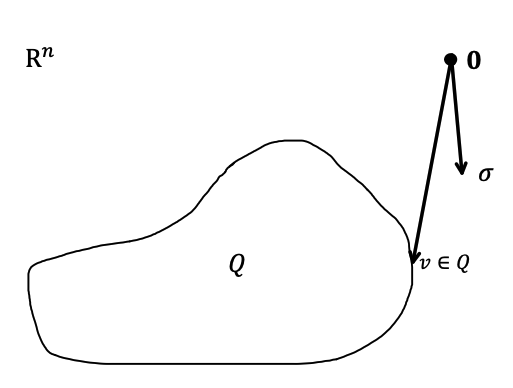
\includegraphics[width=.5\textwidth]{figures/remark2.png}
\end{center}
\caption{We can view empirical Rademacher complexity as the expectation of the maximum inner product between $\sigma$ and $v\in Q$.}
\label{lec6:fig:rs-innerprod}
\end{figure}

Another corollary of this is that the empirical Rademacher complexity doesn't depend on the exact parameterization of $\cF$. For example, suppose we have two parameterizations $\cF = \left\{f(x)=\sum \theta_{i} x_{i} \mid \theta \in \mathbb{R}^{d}\right\}$ and $\cF' = \left\{f(x)=\sum \theta_{i}^{3} \cdot w_{i} x_{i} \mid \theta \in \R^{d}, w \in \mathbb{R}^{d}\right\}$. Since $Q_\cF$ and $Q_{\cF'}$ are the same, we see that $R_S(\cF) = R_S(\cF')$ since our earlier expression for $R_S(\cF)$ only depends on $\cF$ through $Q_\cF$. 

\subsec{Rademacher complexity is translation invariant}
A useful fact is that both empirical Rademacher complexity and average Rademacher complexity are translation invariant. (This is not obvious when thinking of how translation affects the picture in Figure \ref{lec6:fig:rs-innerprod}.)

\begin{proposition}
Let $\cF$ be a family of functions mapping $Z \mapsto \R$ and define $\cF' = \{f'(z) = f(z) + c_0\mid f\in \cF\}$ for some $c_0\in\R$. Then $R_S(\cF) = R_S(\cF')$ and $R_n(\cF) = R_n(\cF')$.
\end{proposition}

\begin{proof}
We will prove here that empirical Rademacher complexity is translation invariant.
\begin{align}
R_S(\cF') &= \E_{\sigma_1,\dots, \sigma_n} \l[ \sup_{f'\in \cF'} \frac{1}{n} \sum^n_{i=1} \sigma_i f(z_i) \r] \\
&= \E_{\sigma_1,\dots, \sigma_n} \l[ \sup_{f\in \cF} \frac{1}{n} \sum^n_{i=1} \sigma_i (f(z_i)+c_0) \r] \\
&= \E_{\sigma_1,\dots, \sigma_n} \l[ \frac{1}{n} \sum^n_{i=1} \sigma_i c_0 + \sup_{f\in \cF} \frac{1}{n} \sum^n_{i=1} \sigma_i f(z_i) \r] \\
&= \E_{\sigma_1,\dots, \sigma_n} \l[\sup_{f\in \cF} \frac{1}{n} \sum^n_{i=1} \sigma_i f(z_i) \r] = R_S(\cF), \label{lec6:eqn:rs-translation}
\end{align}
where \eqref{lec6:eqn:rs-translation} follows because $\E_{\sigma_1,\dots,\sigma_n} \frac{1}{n}\sum_{i=1}^n \sigma_i c_0 = 0$, since the $\sigma_i$'s are Rademacher random variables.
\end{proof}

\sec{Motivation: VC dimension and its limitations}
Now we will instantiate Rademacher complexity for specific cases. We will focus on classification and will be working within the framework of supervised learning stated in Lecture 1. The labels belong to the output space $\mathcal{Y} = \{-1, 1\}$, each classifier is a function $h:\mathcal{X}\to\R$ for all $h \in \cH$, and the prediction is the sign of the output, i.e. $\hat{y} = \sgn(h(x))$. We will look at zero-one loss, i.e. $\err((x,y), h) = \mathbbm{1}(\sgn(h(x))\neq y)$. Note that we can re-express the loss function as
\begin{equation}
\err((x,y), h) = \frac{1-\sgn(h(x))y}{2}.
\end{equation}

The first approach is to reason directly about the Rademacher complexity of $\err$ loss, i.e. considering the family of functions $\cF = \left\{ z = (x, y) \mapsto \err((x, y), h) : h \in \cH \right\}$. Define $Q$ to be the set of all possible outputs on our dataset: $Q=\left\{\left(\sgn\left(h\left(x^{(1)}\right)\right), \dots, \sgn \left(h\left(x^{(n)}\right)\right)\right)\mid  h \in \cH \right\}$. Then, using our earlier remark about viewing the empirical Rademacher complexity as an inner product between $v\in Q$ and $\sigma$, we have
\begin{align}
R_S(\cF) &= \E_{\sigma_1,\dots, \sigma_n} \l[ \sup_{f\in \cF} \frac{1}{n} \sum^n_{i=1} \sigma_i \frac{1-\sgn(h(x^{(i)}))y_i}{2} \r] \\
&= \E_{\sigma_1,\dots, \sigma_n} \l[ \sup_{f\in \cF} \frac{1}{n} \sum^n_{i=1} \sigma_i \frac{\sgn(h(x^{(i)}))}{2} \r] \\
&= \frac{1}{2}\E_{\sigma_1,\dots, \sigma_n} \l[ \sup_{v\in Q} \frac{1}{n} \langle \sigma, v\rangle \r].
\end{align}

Notice that the supremum is now over $Q$ instead of $\cF$. If $n$ is sufficiently large, then it is typically the case that $|Q|>|\cF|$. To see why this is the case, note that each function $f$ corresponds to a single element in $Q$. However, as $n$ increases, $|Q|$ increases as well. For any particular $v\in Q$, notice that $\langle v, \sigma\rangle$ is a sum of bounded random variables, so we can use Hoeffding's inequality to obtain
\begin{equation}
\Pr\left[\frac{1}{n}(\sigma, v) \geq t\right] \leq \exp (-n t^2 / 2).
\end{equation}
Taking the union bound over $v\in Q$, we see that 
\begin{equation}
    \Pr\left[\exists v\in Q \text{ such that } \frac{1}{n}\langle\sigma, v\rangle \geq t\right] \leq |Q| \exp (-nt^2 / 2).
\end{equation}
Thus, with probability at least $1-\delta$, it is true that $\sup _{v \in Q} \frac{1}{n}\langle v, \sigma \rangle \leq \sqrt{\frac{2(\log|Q| + \log (2/\delta))}{n}}$. Similarly, we can show that $\E \left[ \sup _{v \in Q} \frac{1}{n}\langle v, \sigma \rangle \right] \leq O\l(\sqrt{\frac{\log|Q| + \log (2/\delta)}{n}}\r)$ holds.

The key point to notice here is that the upper bound on $R_S(\cF)$ depends on $\log |Q|$. \textit{VC dimension} is one way that we deal with bounding the size of $Q$ We will not delve into the details of this approach (for those interested, see Section 3.11 of \cite{percynotes}). VC dimension, however, has a number of limitations. For one, we will always end up with a bound that depends somehow on the dimension. For linear models, we obtain a bound $\log |Q| \lesssim d \log n$, corresponding to a bound on Rademacher complexity that looks like
\begin{equation}
    R_S(\cF) \leq \tilO \left( \sqrt{\frac{d}{n}} \right),
\end{equation}
so we still have a $\sqrt{d}$ term. This will not be a good bound for high-dimensional models. For general models, we will arrive a bound of the form 
\begin{equation}
    R_S(\cF) \leq \tilO \left( \sqrt{\frac{\text{\# of parameters}}{n}} \right).
\end{equation}
This upper bound only depends on the number of parameters in our model, and does not take into the account the scale and norm of the parameters. Additionally, this doesn't work with kernel methods since the explicit parameterization is possibly infinite-dimensional, and therefore this upper bound becomes useless.

These limitations motivation the use of margin theory, which does take into account the norm of parameters and provides a theoretical basis for regularization techniques such as $L_1$ and $L_2$ regularization.

\sec{Margin Theory}

\subsec{Intuition}
Assume that we are in the same setting as in the previous section. A fundamental problem we face in this setting is that we do not have a continuous loss: everything is discrete in the output space. We need to find a way to reason about the scale of the output. An example of this is logistic regression: the logistic regression model outputs a probability, and while we compare it to the outcome (0 or 1), how close it is to the true output gives us a measure of how confident we are in the prediction.

Figure \ref{lec6:fig:margin} gives similar intuition for linear classifiers. Intuitively, the black line is a "better" decision boundary than the red line because the minimum distance from any point to the black boundary is greater than the minimum distance from any point to the red line. In the next section, we will formalize this intuition by proving that the larger this margin is, the smaller the bound on generalization gap is.

\begin{figure}[h!]
    \begin{center}
  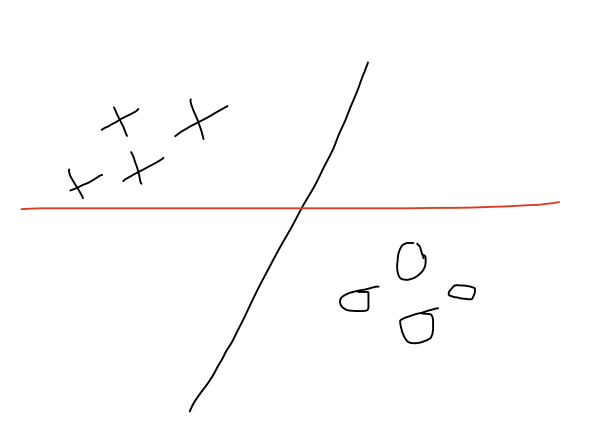
\includegraphics[width=0.5\textwidth]{figures/margin.png}
  \end{center}
  \caption{The red and black lines are two decision boundaries. The X's are positive examples and the O's are negative examples. The black line has a larger margin than the red line, and is intuitively a better classifier.}
  \label{lec6:fig:margin}
\end{figure}

\subsec{Formalizing margin theory}
First, assume that the dataset $\cD = ((x\sp{1}, y\sp{1}), \dots, (x\sp{n}, y\sp{n}))$ is \textit{completely separable}. In other words, there exists some $h_\theta\in\cH$ such that $y^{(i)} = \sgn(h_\theta(x^{(i)}))$ holds for all $( x^{(i)},y^{(i)})\in \cD$. This is not a necessary condition for our final bound but will make the derivation cleaner.

\begin{definition}[(Unnormalized) Margin]
Fix the hypothesis $h_\theta$. The \textit{(unnormalized) margin} for example $(x, y)$ is defined as $\margin(x) = yh_\theta(x)$. Margin is only defined on examples where $\sgn(h_\theta(x)) = y$. (Note that $\margin(x)\geq 0$ because of our assumption of complete separability.)
\end{definition}

\begin{definition}[Minimum margin] Given a dataset $\cD = ((x\sp{1}, y\sp{1}), \dots, (x\sp{n}, y\sp{n}))$, the \textit{minimum margin} over the dataset is defined as $\gamma_{\min} \triangleq \min_{i\in\{1,\dots,|\cD|\}} y^{(i)}h_\theta(x^{(i)})$.
\end{definition}

Our final bound will have the form (generalization gap)$\leq f(\text{margin},\text{parameter norm})$. This is very generic since there are many different bounds we could derive based on what margin we use. For this current setting we are using $\gamma_{\min}$, which is the minimum margin, but in other settings could use $\gamma_{\text{average}}$, which is the average margin of each point in the dataset.

We will begin by introducing the idea of a \textit{surrogate loss}, a loss function which approximates zero-one loss but takes the scale of the margin into account. The \textit{margin loss} (also known as \textit{ramp loss}) is defined as 
\begin{equation}
    \ell_\gamma(t) = \begin{cases} 
      0 & t\geq \gamma \\
      1 & t\leq 0 \\
      1-t/\gamma & 0\leq t\leq \gamma
   \end{cases}
\end{equation}

\begin{figure}[h!]
    \begin{center}
  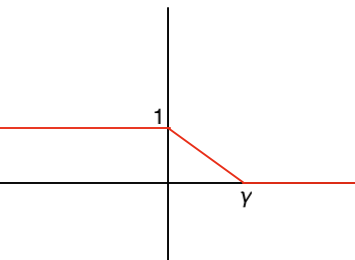
\includegraphics[width=0.5\textwidth]{figures/margin_loss.png}
  \end{center}
  \caption{Plotted margin loss.}
  \label{lec6:fig:marginloss}
\end{figure}

It is plotted in Figure \ref{lec6:fig:marginloss}. For convenience, define $\ell_\gamma((x,y), h) \triangleq \ell_\gamma(yh(x))$. We can view $\ell_\gamma$ as a continuous version of $\err$ while being more sensitive to the scale of the margin on $[0,\gamma]$. Notice that $\err$ is always less than or equal to the $\ell_\gamma$ when $\gamma\geq 0$, i.e.
\begin{equation}
    \err((x,y), h)\leq \ell_\gamma ((x,y), h)
\end{equation}
holds for all $(x,y)\sim P$. Taking the expectation over $(x,y)$ on both sides of this inequality, we see that
\begin{equation}
    L(h) = \E_{(x,y)\sim P} \left[ \err((x,y), h) \right] \leq \E_{(x,y)\sim P} \left[ \ell_\gamma ((x,y), h) \right].
\end{equation}

Therefore, the population loss is bounded by the expectation of the margin loss, and so it is sufficient to bound the expectation of the margin loss in order to bound the population loss.

Define the population and empirical version of the margin loss:
\begin{equation}
L_\gamma(h) = \E_{(x,y)\sim P}\l[ \ell_\gamma((x,y), h)\r], \quad \hat{L}_\gamma(h) = \sum_{i=1}^n\l [\ell_\gamma((x^{(i)},y^{(i)}), h)\r].
\end{equation}

By Corollary \ref{lec6:cor:ggap-rsbound}, we see that with probability at least $1-\delta$ that
\begin{equation}
L_\gamma(h) - \hat{L}_\gamma(h)\leq 2R_S(\cF) + 3\sqrt{\frac{\log (2/\delta)}{2n}},
\end{equation}
where $\cF = \{(x,y)\mapsto \ell_\gamma((x,y), h)\mid h\in\cH\}$. Note that if we set $\gamma\leq \gamma_{\min}$, then $\hat{L}_{\gamma}(h) = 0$. This follows because by definition of $\gamma_{\min}$, $y^{(i)}h(x^{(i)})\geq \gamma_{\min}$ for any $(x^{(i)}, y^{(i)})\in \cD$. As a result, $\ell_\gamma((x^{(i)}, y^{(i)}), h) = \ell_\gamma(y^{(i)}h(x^{(i)})) = 0$ holds. Therefore, it suffices to bound $R_S(\cF)$.

We will now use \textit{Talagrand's lemma} to bound $R_S(\cF)$ in terms of $R_S(\cH)$ to remove any dependence on the loss function from the upper bound. 
 
\begin{lemma}{(Talagrand's lemma)}
Let $\phi:\R\to\R$ be a $\kappa$-Lipschitz function. Then \begin{equation}
    R_S(\phi\circ \cH)\leq \kappa R_S(\cH),
\end{equation} 
where $\phi\circ\cH = \{z\mapsto \phi(h(z))\mid h\in\cH\}$.
\end{lemma}

We can use Talagrand's lemma directly with $\phi(t) = \ell_\gamma(t)$, which is $\frac{1}{\gamma}$-Lipschitz. We can express $\cF$ as $\cF=\ell_\gamma\circ\cH'$ where $\cH' = \{(x,y)\to yh(x)\mid h\in\cH\}$. Applying Talagrand's lemma, we see that

\begin{align}
R_S(\cF) &\leq \frac{1}{\gamma}R_S(\cH') \\
&= \frac{1}{\gamma}\E_{\sigma_1,\dots, \sigma_n} \l[ \sup_{h\in \cH} \frac{1}{n} \sum^n_{i=1} \sigma_i y^{(i)}h(x^{(i)}) \r] \\
&= \frac{1}{\gamma}\E_{\sigma_1,\dots, \sigma_n} \l[ \sup_{h\in \cH} \frac{1}{n} \sum^n_{i=1} \sigma_i h(x^{(i)})  \r] \\
&= \frac{1}{\gamma}R_S(\cH).
\end{align}

Putting this all together, we have shown that for $\gamma \leq \gamma_{\min}$,
\begin{align}
\Err(h) \leq L_\gamma(h) &\leq 0 + O \left( \frac{R_S(\cH)}{\gamma} \right) + \tilO \left( \sqrt{\frac{\log (2 / \delta)}{2n}} \right) \\
&= O \left( \frac{R_S(\cH)}{\min_i y\sp{i} h(x\sp{i}) } \right) + \tilO \left( \sqrt{\frac{\log (2 / \delta)}{2n}} \right).
\end{align}

In the next lecture, we will talk about how we can bound $R_S(\cH)$ by the norms for linear models, two-layer neural networks and multi-layer neural networks. 

\begin{remark}
Note there is a subtlety here. If we think of the dataset as random, it follows that $\gamma_{\min}$ is a random variable. Consequently, the $\gamma$ we choose to define the hypothesis class is random, which is not a valid choice when thinking about Rademacher complexity! Technically we cannot apply Talagrand's lemma with a random $\kappa$ (which we took to be $1/\gamma$). Also, when we used concentration inequalities, we implicitly assume that the $\ell_\gamma((x\sp{i}, y\sp{i}), h)$ are independent of each other. That is not the case if $\gamma$ is dependent on the data.

How can we address this? The idea is to do another union bound over $\gamma$. Choose a family $\Gamma = \left\{ 2^k: k \in [-B, B] \right\}$ for some $B$. For every fixed $\gamma \in \Gamma$, we prove the theorem that
\begin{align}
\Err(h) \leq \hatL_\gamma (h) + O \left( \frac{R_S(\cH)}{\gamma} \right) + \tilO \left( \frac{1}{\sqrt{n}} \right).
\end{align}
\end{remark}

We can then take a union bound over all $\gamma \in \Gamma$. Next, choose the largest $\gamma \in \Gamma$ such that $\gamma \leq \gamma_{\min}$. For this value of $\gamma$ we have $\hatL_\gamma (h) = 0$ and $O \left( \frac{R_S(\cH)}{\gamma} \right) = O \left( \frac{R_S(\cH)}{\gamma_{\min}} \right)$. \tnotelong{make this part more formal. }

	
	%    Include main chapters here.
	%\include{}
	\appendix
	%    Include appendix "chapters" here.
	
	
	%\backmatter
	%    Bibliography styles amsplain or harvard are also acceptable.
	\bibliographystyle{amsalpha}
	\bibliography{bibliography}
	%    See note above about multiple indexes.
%	\printindex
	
	\end{document}
	
	%-----------------------------------------------------------------------
	% End of amsbook-template.tex
	%-----------------------------------------------------------------------
